\documentclass[letterpaper,11pt]{article}
\oddsidemargin -1.0cm \textwidth 17.5cm

\usepackage[utf8]{inputenc}
\usepackage[activeacute,spanish]{babel}
\usepackage{amsfonts,setspace}
\usepackage{amsmath}
\usepackage{amssymb, amsmath, amsthm}
\usepackage{comment}
\usepackage{amssymb}
\usepackage{dsfont}
\usepackage{anysize}
\usepackage{multicol}
\usepackage{enumerate}
\usepackage{graphicx}
\usepackage[left=1.5cm,top=2cm,right=1.5cm, bottom=1.7cm]{geometry}
\setlength\headheight{1.5em} 
\usepackage{fancyhdr}
\usepackage{multicol}
\usepackage{hyperref}
\usepackage{wrapfig}
\pagestyle{fancy}
\fancyhf{}
\renewcommand{\labelenumi}{\normalsize\bfseries P\arabic{enumi}.}
\renewcommand{\labelenumii}{\normalsize\bfseries (\alph{enumii})}
\renewcommand{\labelenumiii}{\normalsize\bfseries \roman{enumiii})}

\begin{document}

\fancyhead[L]{\itshape{Facultad de Ciencias F\'isicas y Matem\'aticas}}
\fancyhead[R]{\itshape{Universidad de Chile}}

\begin{minipage}{11.5cm}
    \begin{flushleft}
        \hspace*{-0.6cm}\textbf{FI1000-5 Introducción a la Física Clásica}\\
        \hspace*{-0.6cm}\textbf{Profesora:} Paulina Lira\\
        \hspace*{-0.6cm}\textbf{Auxiliares:} Alejandro Silva, Felipe Kaschel, Juan Cristóbal Castro\\
    \end{flushleft}
\end{minipage}

\begin{picture}(2,3)
    \put(366,-4){
\includegraphics[scale=0.9]{2020-1/Imágenes/logo/dfi-fcfm.pdf}}
\end{picture}

\begin{center}
	\LARGE \bf Auxiliar \# 10   \\
\end{center}

\vspace{-1cm}
\begin{enumerate}\setlength{\itemsep}{0.4cm}

\rfoot[]{pág. \thepage}

\item[]

\item En un parque de entretenciones un carro de masa $m$ se desliza por una rampa sin roce desde una altura $h$, partiendo inicialmente desde el reposo. El carro, luego de bajar por la rampa, ingresa a un \textit{loop} de radio~$R$ tal que $2R<h$. Emergiendo del \textit{loop}, el carro ingresa a la región de frenado, donde en un trayecto de largo $L$ se tiene un coeficiente de roce cinético $\mu_c$. Sin embargo, el carro no alcanza a detenerse durante la primera pasada, siguiendo de largo para colisionar con un resorte de constante $k$. El carro vuelve a ingresar a la región de frenado y finalmente se detiene en el centro de ella.
\begin{enumerate}
    \item Encuentre la velocidad del carro en el punto $B$
    \item Encuentre la máxima compresión que alcanza a tener el resorte.
    \item Encuentre una expresión para $\mu_c$
\end{enumerate}

\begin{figure}[h!]
    \centering
    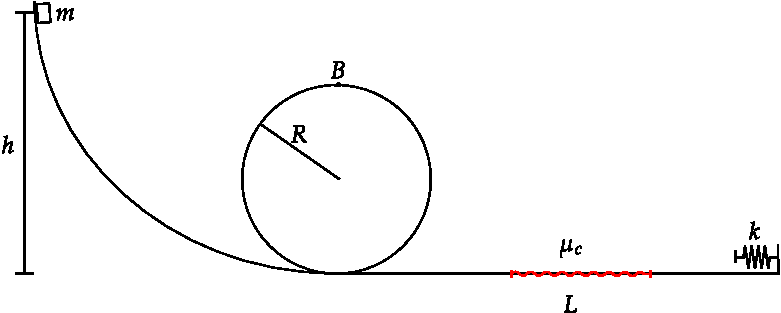
\includegraphics[scale=0.65]{2020-1/Imágenes/aux10/raptor.pdf}
\end{figure}

\item Una masa $m$ resbala, sin roce y debido a la gravedad, por la superficie de una semiesfera de radio $R$. La masa parte desde la cúspide sin velocidad inicial. Sea $P$ el punto en el cual la masa se separa de la semiesfera. Encuentre el ángulo de elevación $\theta_0$ del punto P.

\begin{figure}[h!]
    \centering
    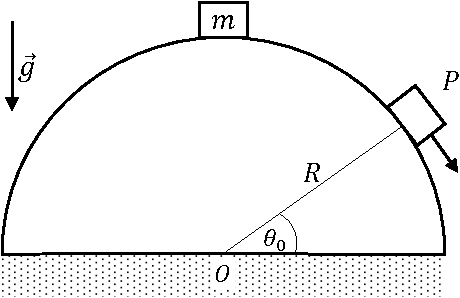
\includegraphics[scale=0.65]{2020-1/Imágenes/aux10/semiesfera_masa.pdf}
\end{figure}

\end{enumerate}
\end{document}